%
% File acl2019.tex
%
%% Based on the style files for ACL 2018, NAACL 2018/19, which were
%% Based on the style files for ACL-2015, with some improvements
%%  taken from the NAACL-2016 style
%% Based on the style files for ACL-2014, which were, in turn,
%% based on ACL-2013, ACL-2012, ACL-2011, ACL-2010, ACL-IJCNLP-2009,
%% EACL-2009, IJCNLP-2008...
%% Based on the style files for EACL 2006 by 
%%e.agirre@ehu.es or Sergi.Balari@uab.es
%% and that of ACL 08 by Joakim Nivre and Noah Smith

\documentclass[11pt,a4paper]{article}
\usepackage[hyperref]{acl2019}
\usepackage{times}
\usepackage{latexsym}
\usepackage{amsmath}
\usepackage{graphicx}
\usepackage{caption}
\usepackage{subcaption}
\usepackage{hyperref}

\usepackage{relsize}
\renewcommand*{\UrlFont}{\smaller\relax}


\DeclareMathOperator*{\argmax}{arg\,max}
\DeclareMathOperator*{\argmin}{arg\,min}
\usepackage{enumitem}


\usepackage{url}

\aclfinalcopy % Uncomment this line for the final submission
%\def\aclpaperid{***} %  Enter the acl Paper ID here

%\setlength\titlebox{5cm}
% You can expand the titlebox if you need extra space
% to show all the authors. Please do not make the titlebox
% smaller than 5cm (the original size); we will check this
% in the camera-ready version and ask you to change it back.
\newcommand\BibTeX{B\textsc{ib}\TeX}

\title{Concept Tagging for the Movie Domain by using Tranfer Learning and Named Entity Recognition.}

\author{Giovanni De Toni (197814) \\
  University of Trento \\ Via Sommarive, 9, 38123 Povo,Trento TN\\
  \texttt{giovanni.detoni@studenti.unitn.it}}

\date{}

\begin{document}
\maketitle

\begin{abstract}
Neural Networks have produced remarkable results in many Natural Language Processing tasks, for example, when tasked to assigning concepts to words of a sentence. Their successes are made possible by employing good word representations (embeddings) which a Neural Network can understand. This work evaluates several newly developed pre-trained embeddings (ELMo, BERT and ConceptNet) on the task of tagging sequences from the movie domain. We then compare the measurements with previous results of the literature.
\end{abstract}

\section{Introduction}
Concept Tagging sequence is a classical problem in 
the NLP field. It consists of assigning to each word 
of a sentence a given concept which represents the 
meaning of that word (e.g., ``\textit{star wars}" is 
a movie title, hence the concept ``
\textit{movie.title}"). Over the past years, it was 
extensively studied and several techniques were 
developed such to efficiently tag words given a pool 
of concepts. The most basic methods are statistical 
language models (e.g., Weight Finite State Automa) 
which are easy to train and yield quite impressive 
results with a little tuning. However, with the rise 
of recurrent neural networks, we can now train 
models which have better performances than their 
statistic counterparts. Moreover, thanks to the use 
of specific word embeddings (e.g., word2vec, GloVe, 
ELMo etc.), we can boost the performances even more.
This work takes as a starting point a previous work 
on the topic \cite{gobbi} and it tries to improve 
the results of some of the neural models presented 
there, by adding new features (NER and POS tags) and 
by trying to employ more intelligent embeddings 
(ELMo, BERT and ConceptNet). The report is 
structured as follow: the second section describe 
the models used for the experiments, the third 
section describes the choosen embeddings. The forth 
and fitfth sections describe the analysis of the 
corpora and the embeddings. Ultimately,  the sixth 
and seventh section reports the experiments 
performed and the conclusions.  	

\section{Models}

To evaluate how the performance changes with respect 
to the previous results we selected two models from 
the original work. We concentrated on the neural 
networks approaches by selecting the ones which held 
the best results over the test set. We chose the 
following architectures: LSTM and LSTM-CRF.  
Moreover, we extended the features used by the 
various models by providing also the Part-of-Speech 
tags and the Named Entities Recognition (NER) 
entities as one-hot-encoded vectors.
Long-Short Term Memor (LSTM) \cite{lstm} is a model 
which extends and improve the previous RNN by 
solving the vanishing/exploding gradients problem. 
We tested a simple LSTM which receives in input the 
embeddings of the words concatenated with the new 
features. Moreover, we tested another LSTM model 
which uses also the characters embeddings obtained 
using a convolutional layer (LSTM-CHAR-REP). 
We experimented also with the LSTM-CRF model \cite{
yao2014recurrent, DBLP:journals/corr/HuangXY15} in 
which the LSTM provides the class scores for each 
token and then the Viterbi algorithm is used to 
determine the labels at a global level.  Again, this 
model was also tested by adding the new features 
concatenated to the word embeddings. Moreover, an 
LSTM-CRF version extended with the characters 
convolution was also evaluated (LSTM-CRF-CHAR-REP).

\section{Embeddings}

As a first step to improve the performances of the previous work we concentrated on evaluating several recently proposed pre-trained language models to produce words representations. Generally speaking, language representations can be either \textit{context-free} or \textit{contextual}. 
Context-free means that the word representation is generated without looking at the context in which the word is used. For instance, the word ``\textit{season}" may have different meanings with respect to the context in which it is placed (e.g., ``\textit{Summer is my favourite season}" and ``\textit{Add some season to the chicken and then serve}"), but in a context-free model it will get the same representation (embedding). A contextual representation takes care also of the context in which a word is used.
Moreover, the contextual representations can be further divided into two other categories: \textit{unidirectional} or \textit{bidirectional}. 
A unidirectional model contextualizes a given term by just looking at the words on the right (or on the left) of it.  A bidirectional model instead looks both on the left and on the right of the target word before producing a representation. There are also \textit{swallow bidirectional models} which combine two unidirectional models (one for the left side and one for the right side) to give a more complete representation. In our work, we tested three different embeddings, one for each category (context-free, contextual swallow bidirectional and contextual bidirectional): \textit{ConceptNet}, \textit{ELMo} and \textit{BERT}.

\begin{figure*}[!ht]
\begin{subfigure}{0.5\linewidth}
  \centering
  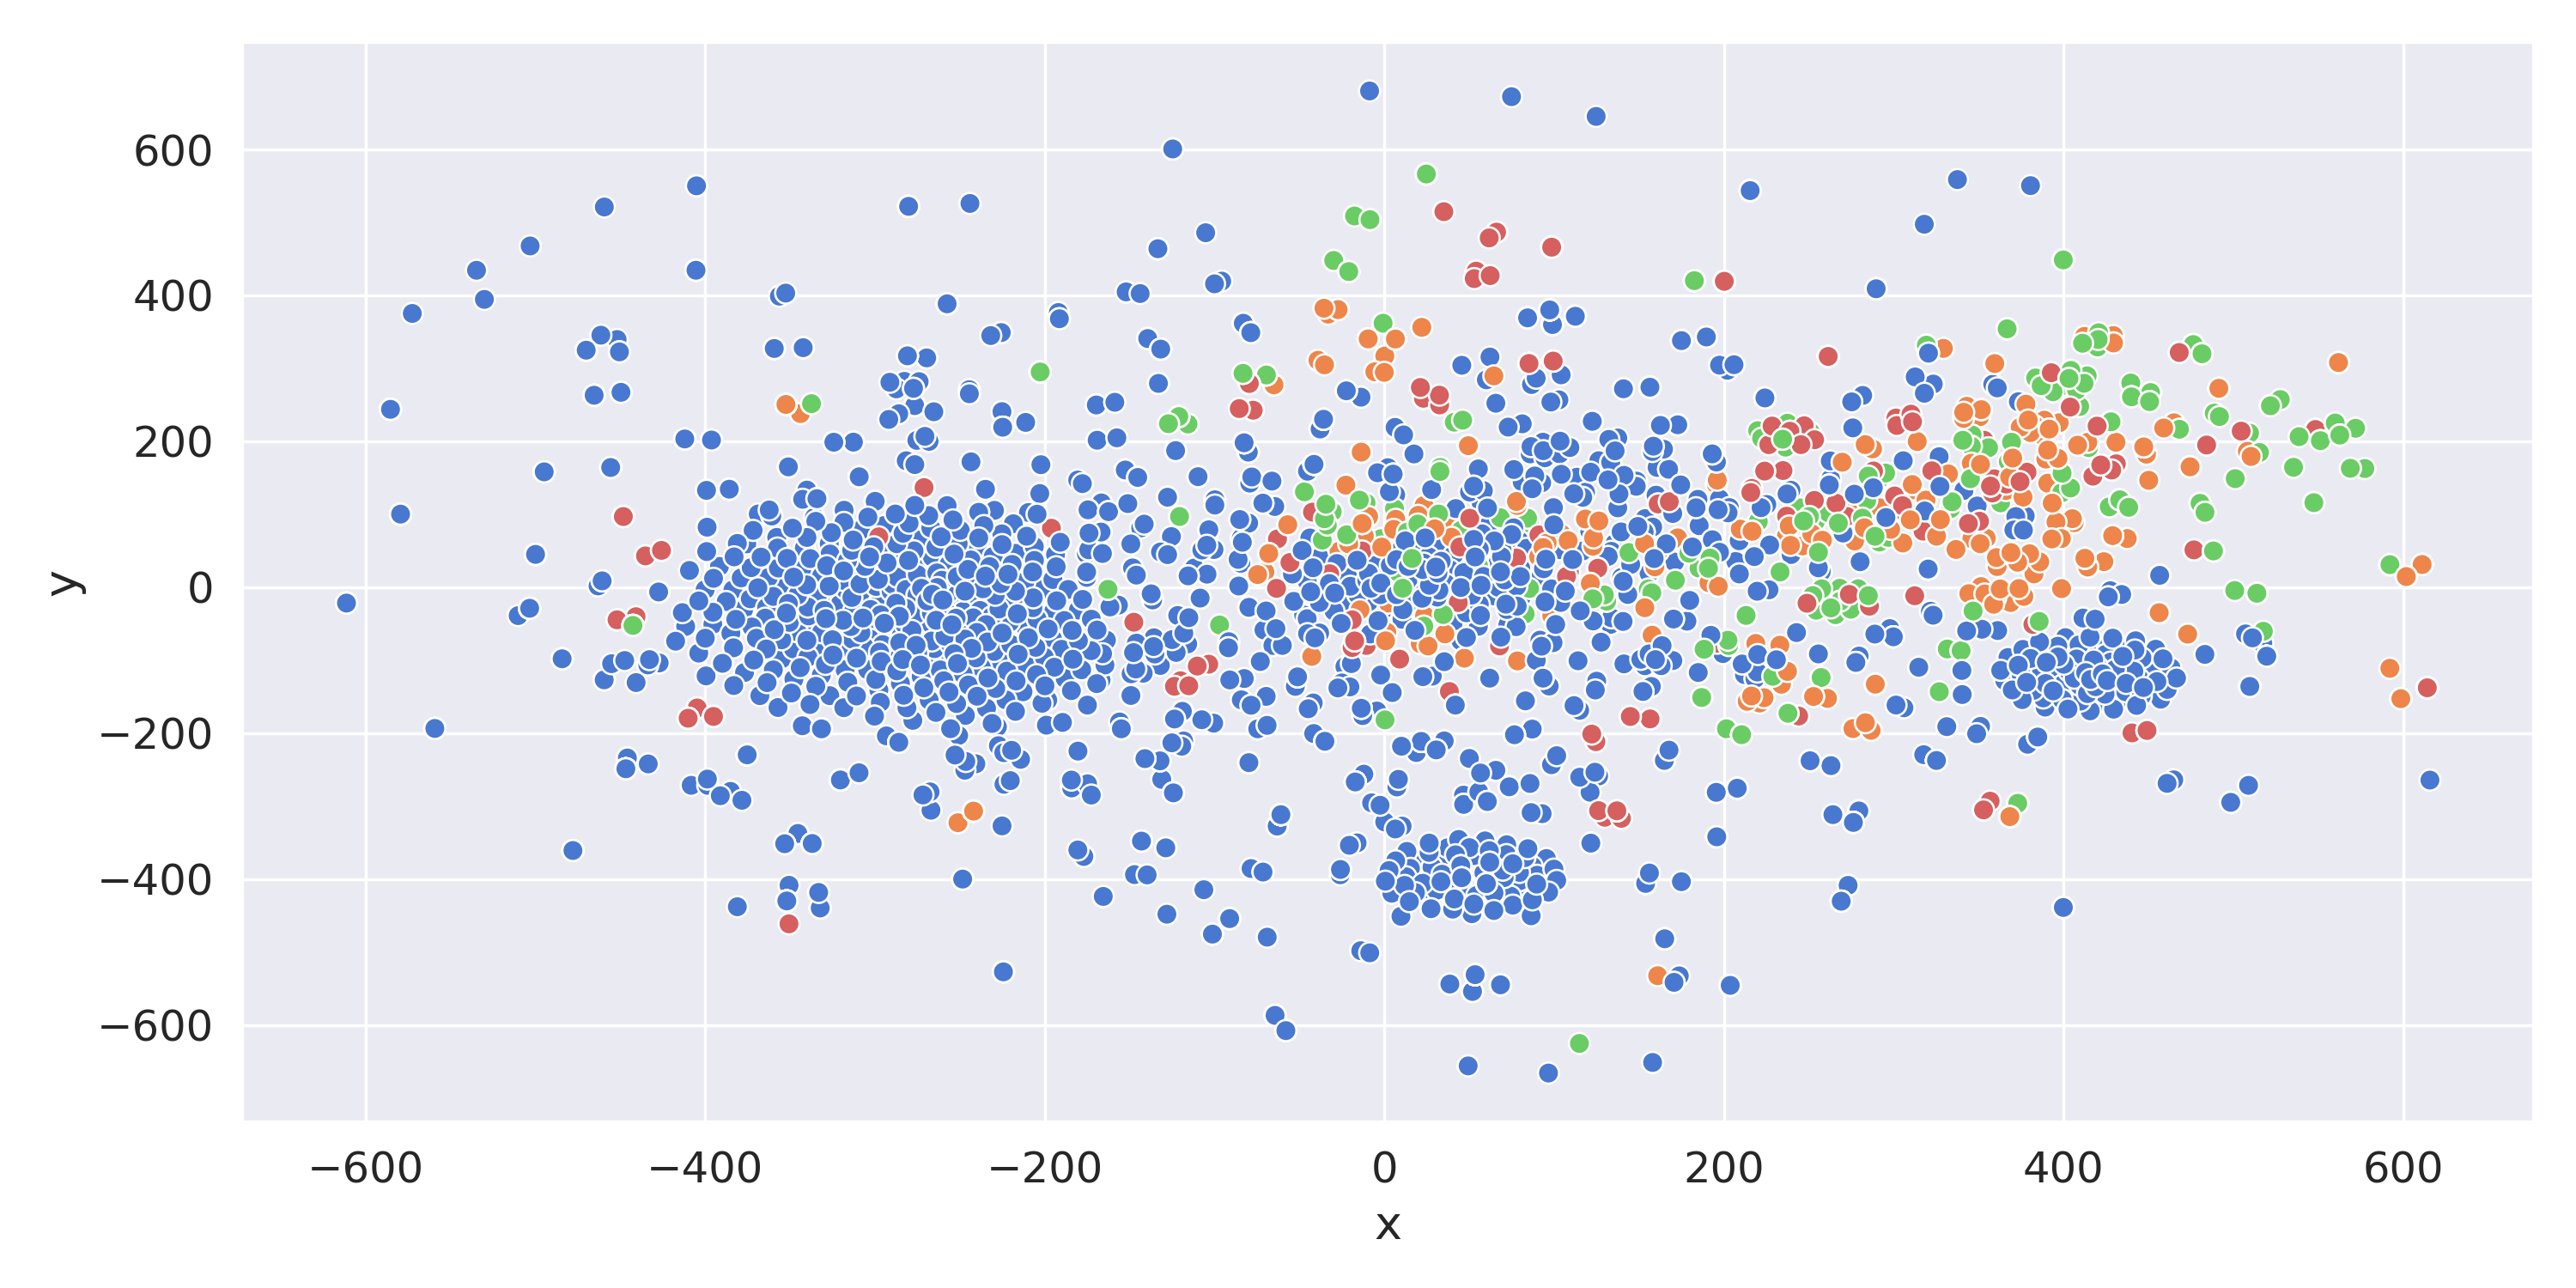
\includegraphics[width=\linewidth]{img/word2vec-embeddings.png}
  \caption{Default Embeddings}
  \label{fig:sfig1}
\end{subfigure}%
\begin{subfigure}{0.5\linewidth}
  \centering
  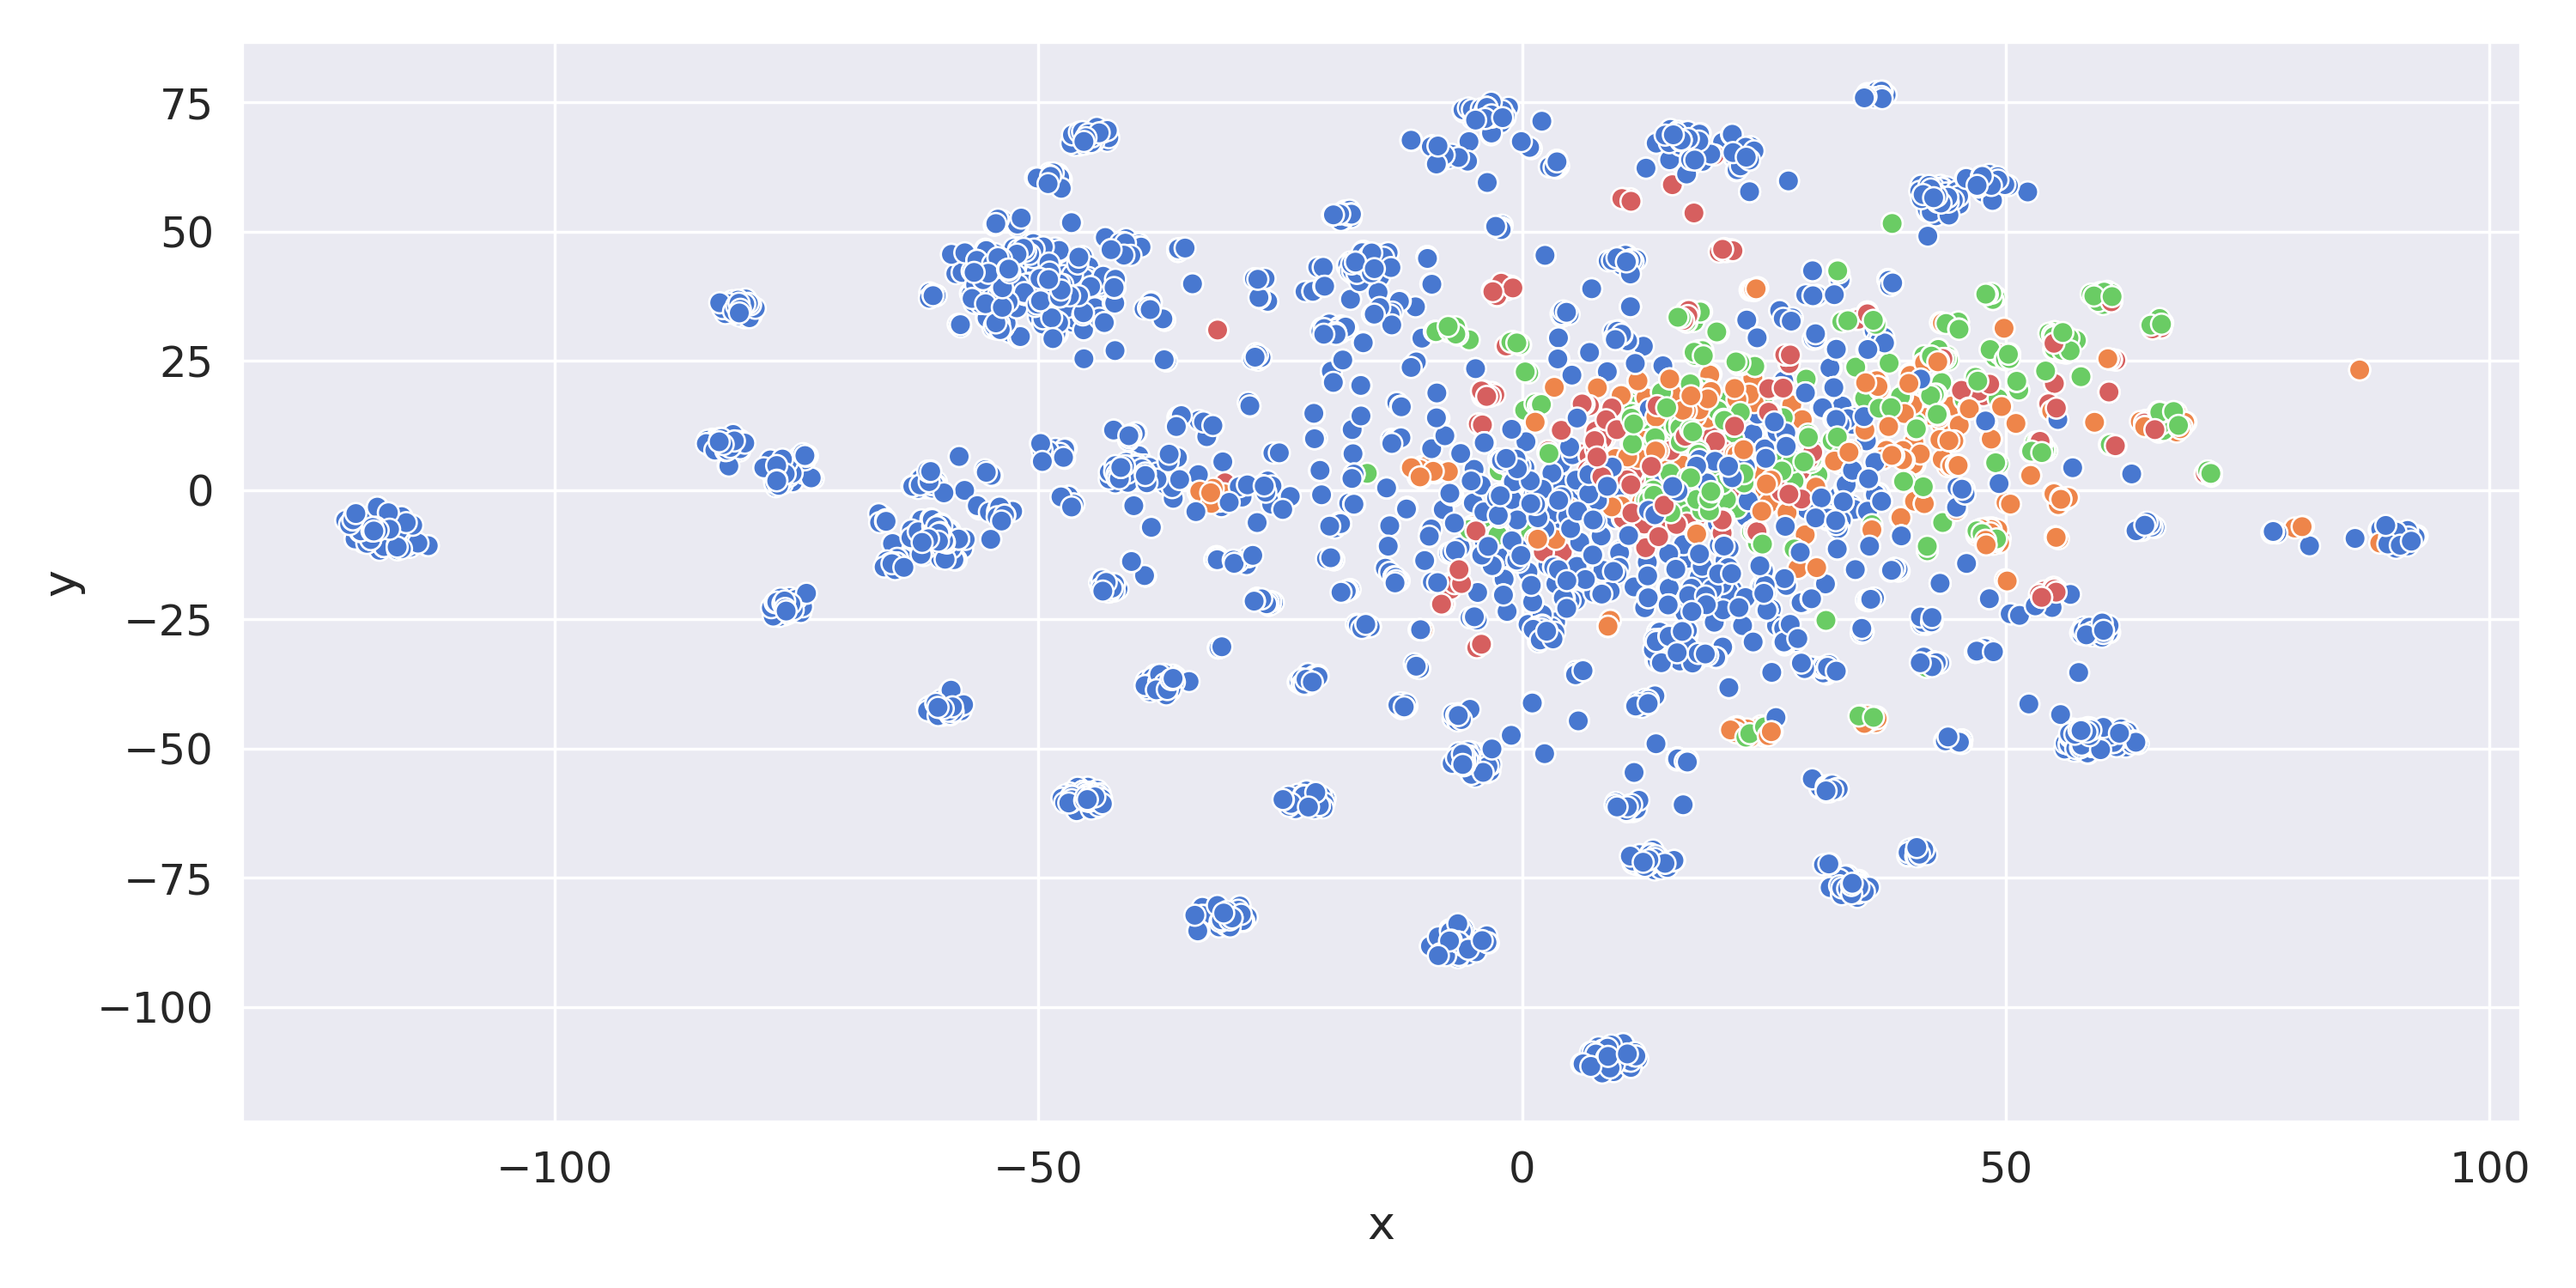
\includegraphics[width=\linewidth]{img/elmo-embeddings.png}
  \caption{Elmo Embeddings}
  \label{fig:sfig2}
\end{subfigure}\\
\begin{subfigure}{0.5\linewidth}
  \centering
  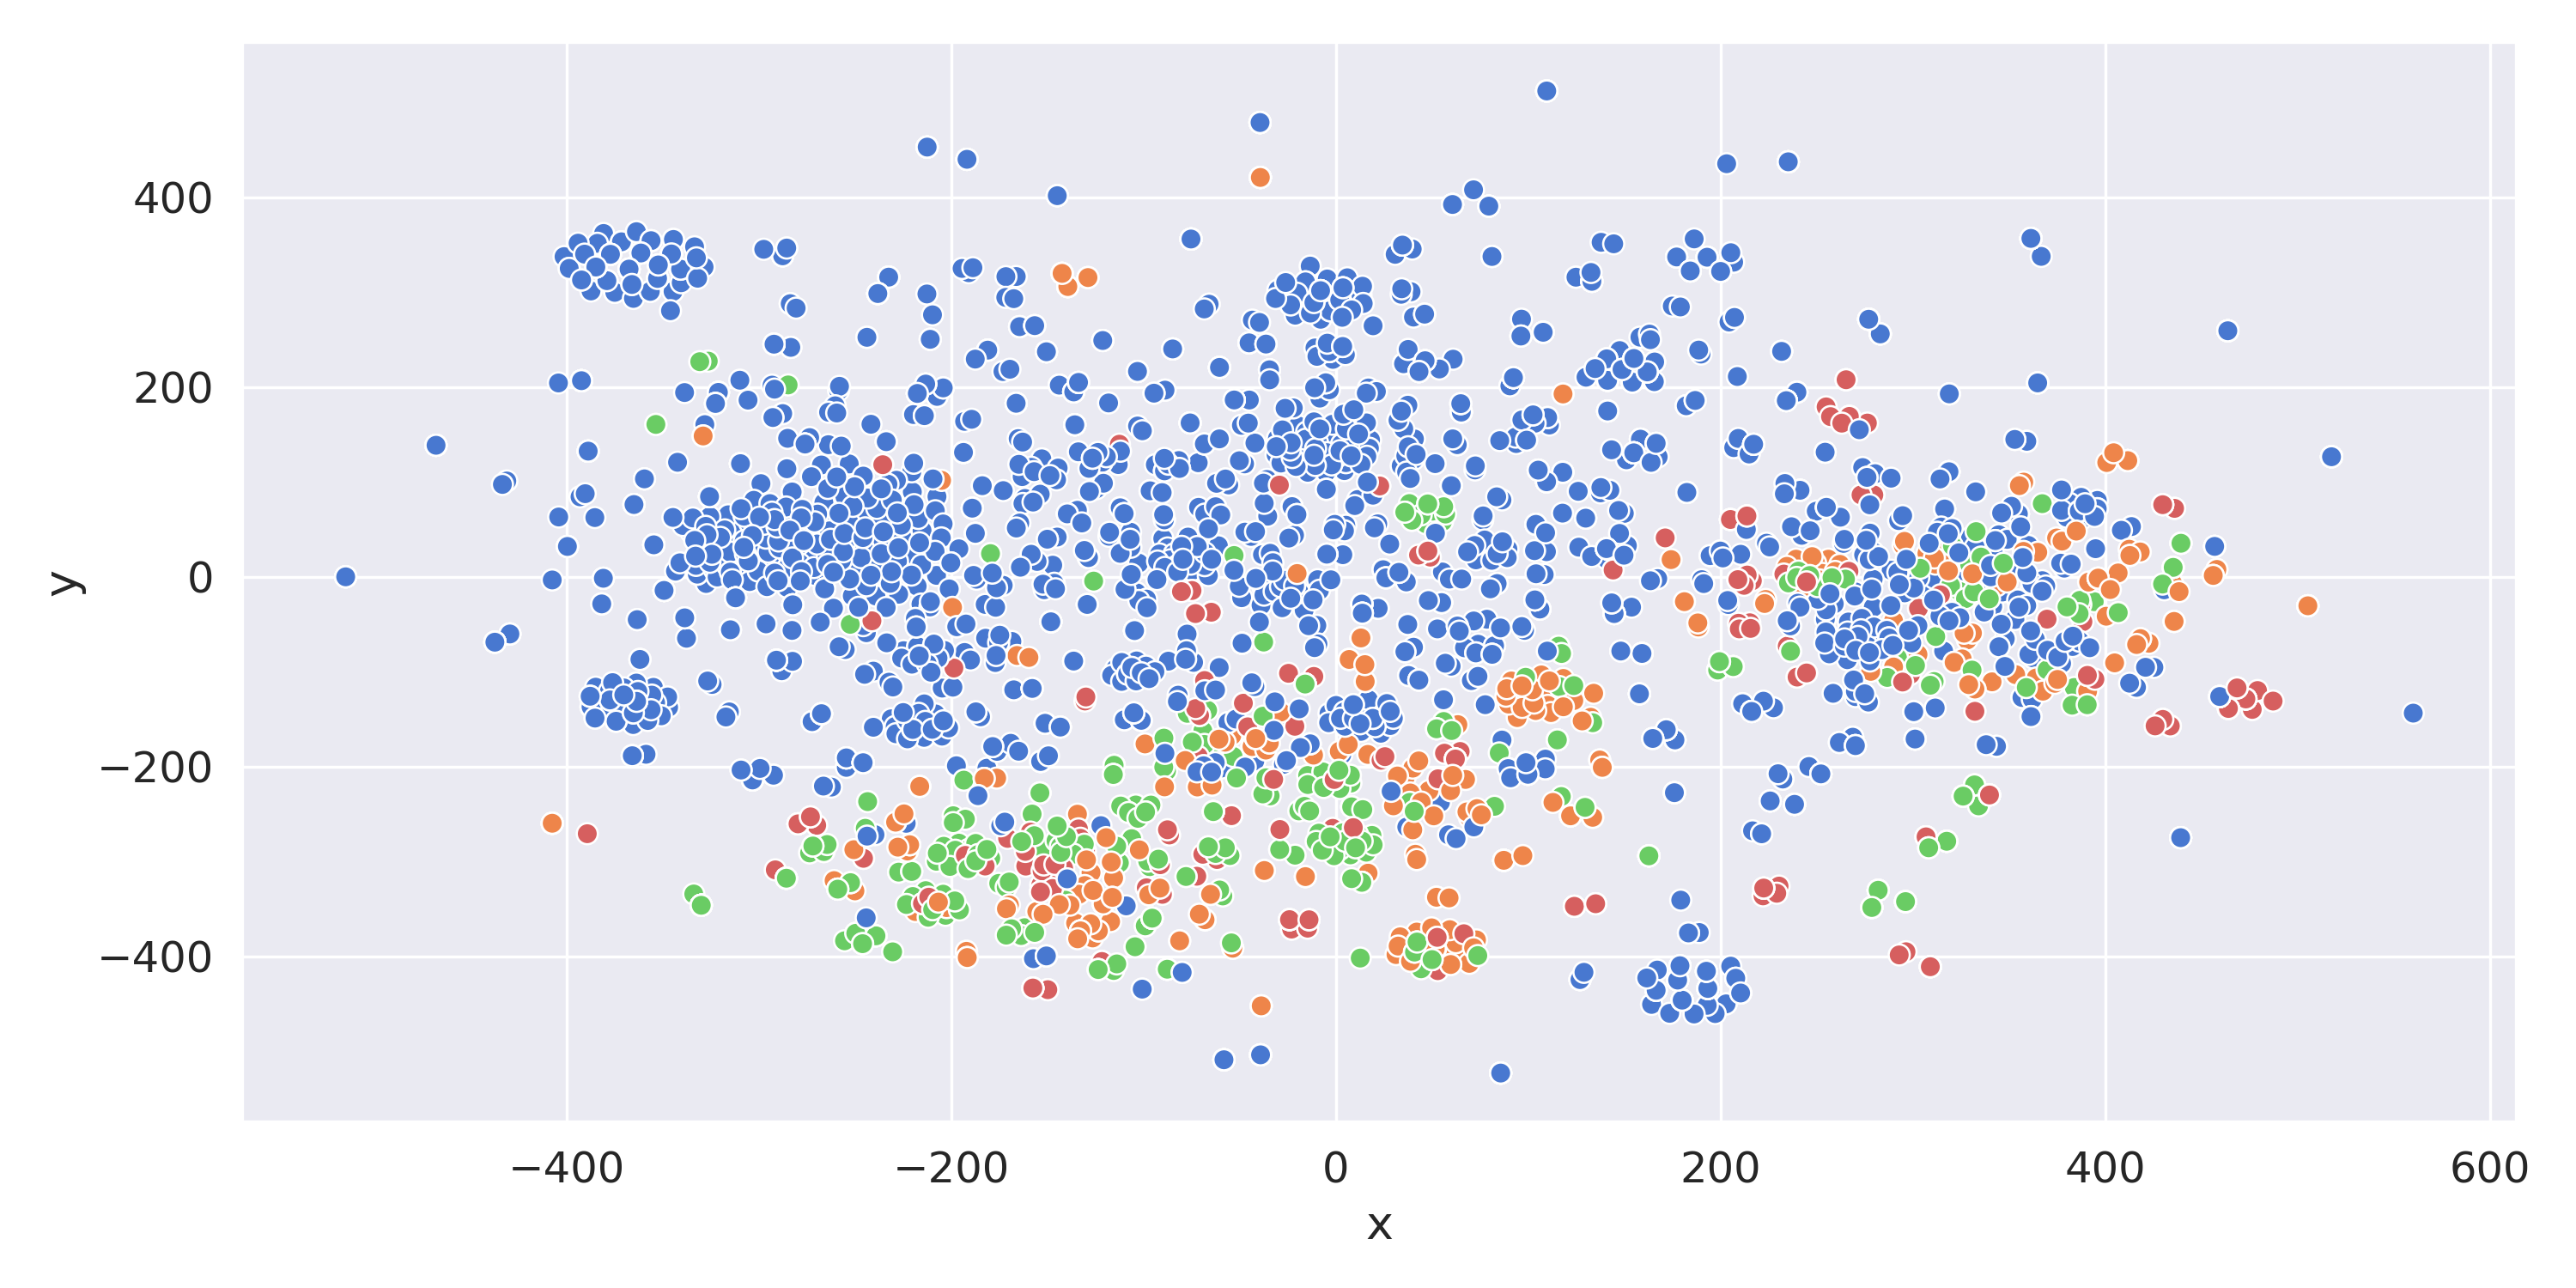
\includegraphics[width=\linewidth]{img/bert-embeddings.png}
  \caption{Bert Embeddings}
  \label{fig:sfig2}
\end{subfigure}%
\begin{subfigure}{0.5\linewidth}
  \centering
  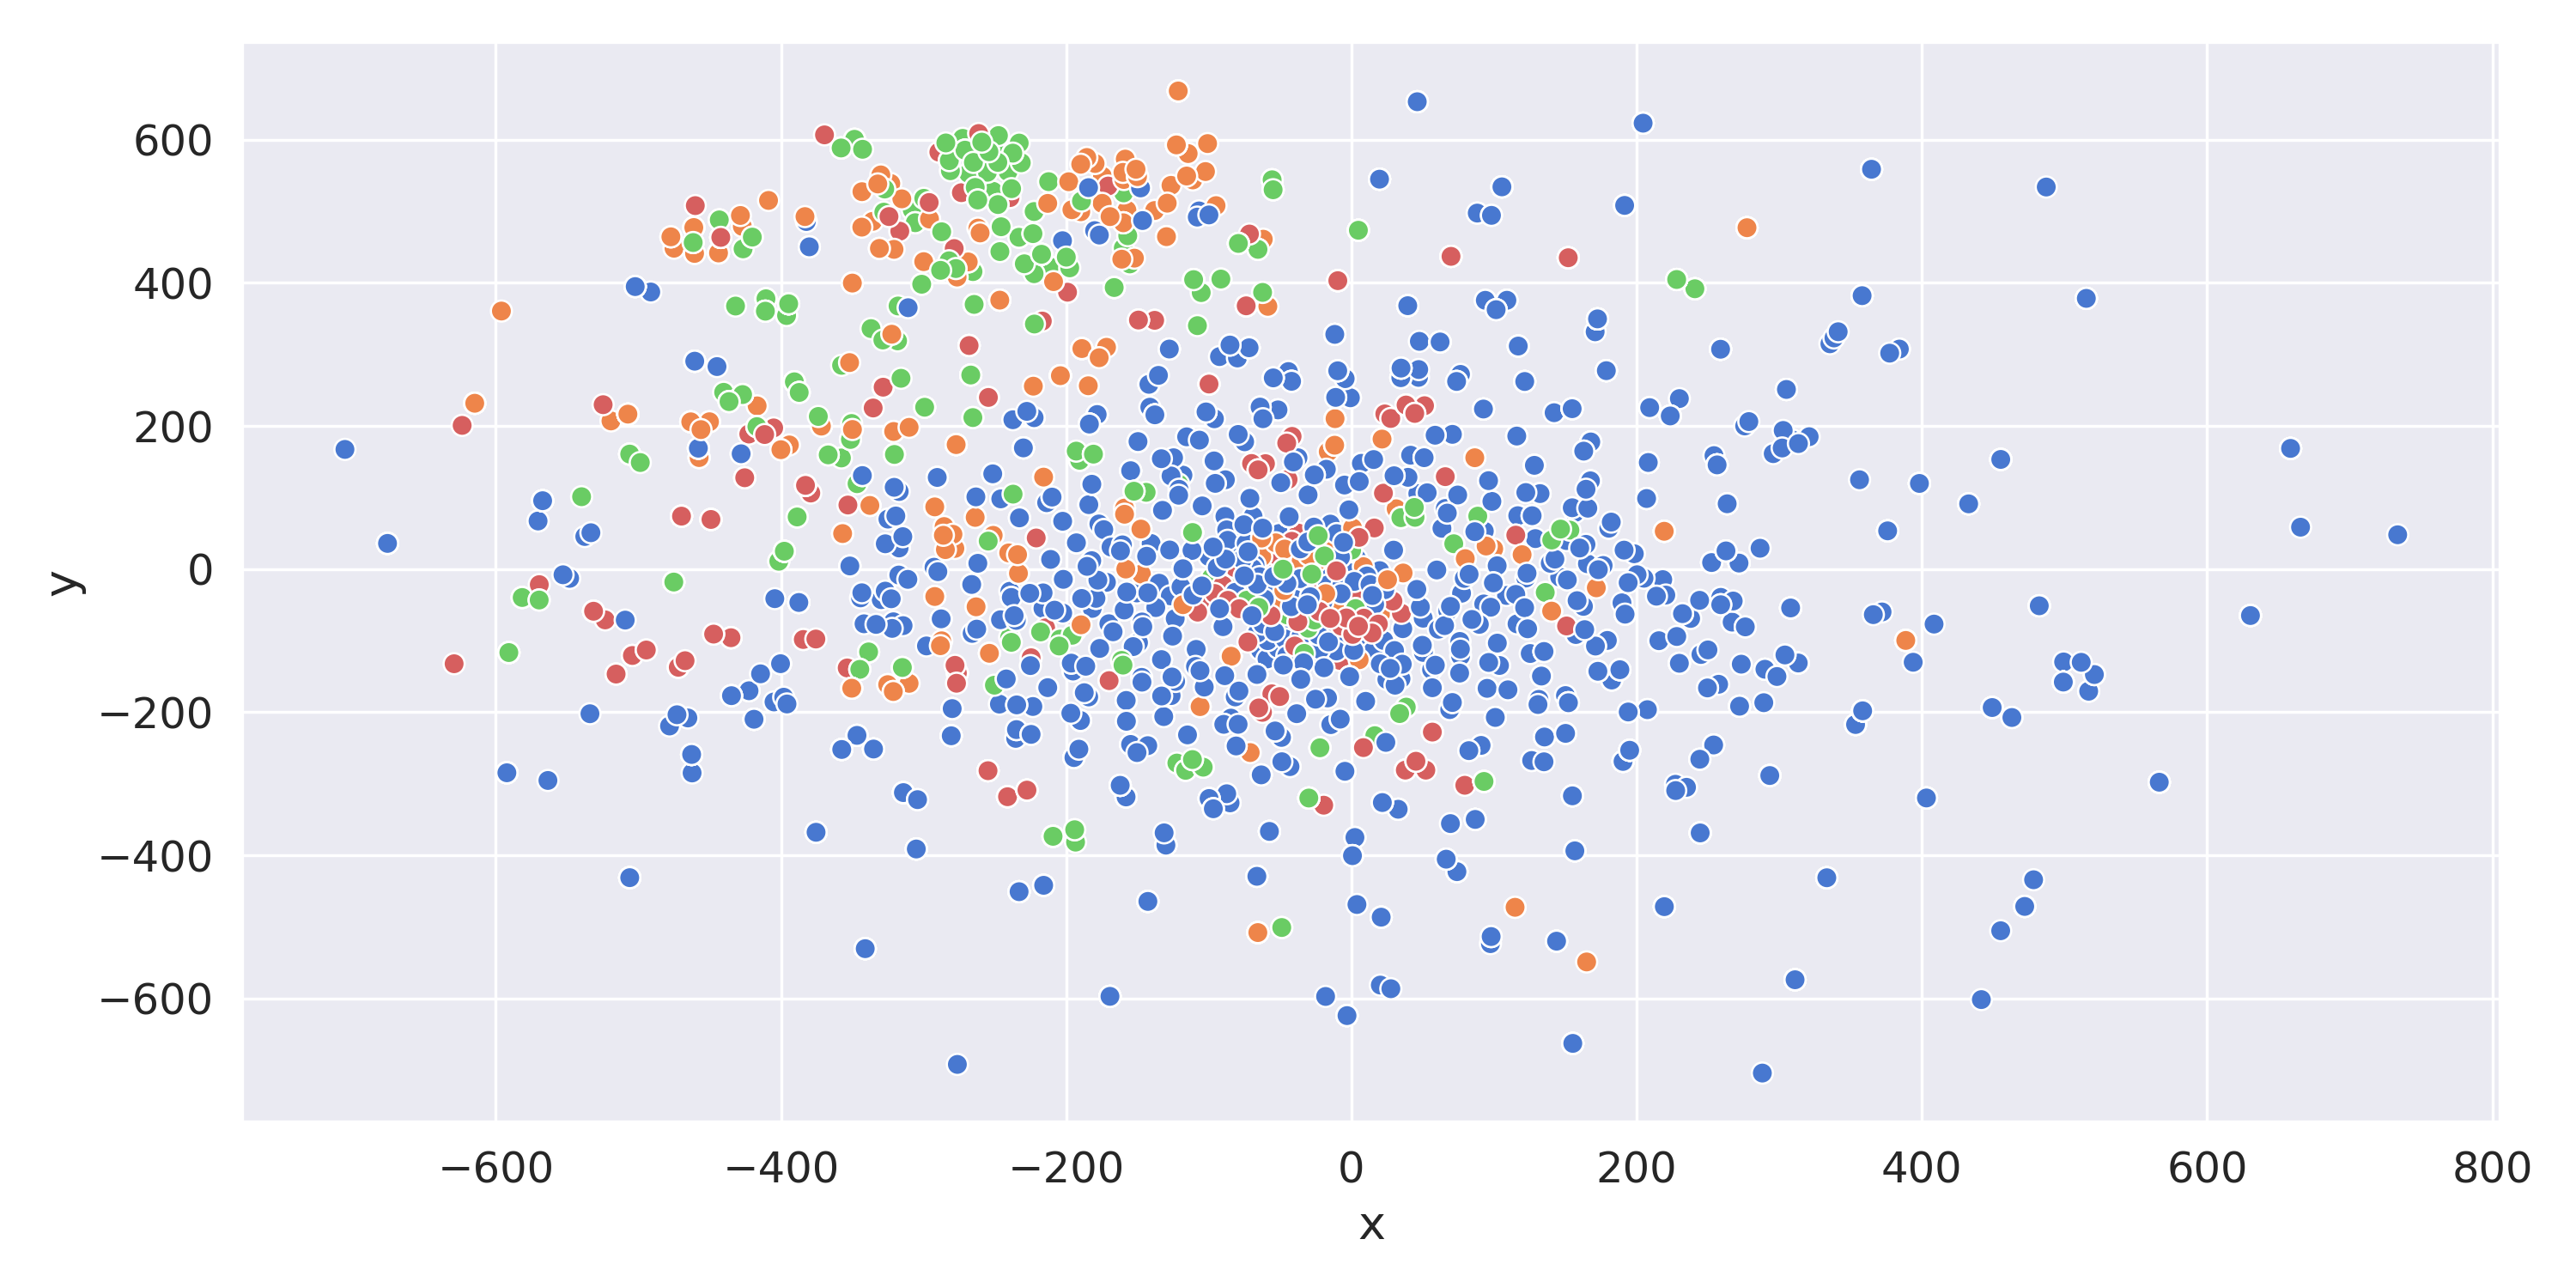
\includegraphics[width=\linewidth]{img/conceptnet-embeddings.png}
  \caption{ConceptNet Embeddings}
  \label{fig:sfig2}
\end{subfigure}
\caption{These plots shows the embeddings representation of the four major concepts of the train dataset. Namely, movie.name (blue), actor.name (orange), producer.name (red) and director.name (green). We can clearly see how some embeddings enable much nicer clusters for some concepts, while others seems not to be able to do it.}
\label{fig:fig}
\end{figure*}

\subsection{ConceptNet}
ConceptNet Numberbatch \cite{speer2017conceptnet} is a context-free language model. It is a set of word embeddings and it was made by combining previously existing models, namely, GloVe \cite{pennington2014glove}, word2vec \cite{mikolov2013efficient} and OpenSubtitles 2016 \cite{Lison2016OpenSubtitles2016EL}. Moreover, it leverages the data of the ConceptNet knowledge graph to enrich its representation. The authors reached this goal by using a retrofitting procedure to adjust the word embedding matrix by using their knowledge graph. Thanks to this procedure, ConceptNet is also intrinsically multilingual since this method pushes the model to use the same embedding space both for English words and words in different languages (since they share the same meaning).  This work uses the Numberbatch 19.08 English-only model \footnote{\url{https://github.com/commonsense/conceptnet-numberbatch}} which contains 516782 embeddings with a dimension of 300.

\subsection{ELMo}
ELMo \cite{Peters:2018} is a deep contextualized word representation which captures both syntactic, semantic and polysemy characteristics of a given word. It uses a deep shallow bidirectional language model (biLM) trained on a large corpus. The ELMo method differs from the classical context-free approaches because each word embedding is obtained by looking at the entire input sentence. The generated representation are deep because they are a function of all the layers of the biLM. Moreover, each layer models certain features of the given word. The original work states that the higher-level LSTM states capture context-dependent aspects of the word meaning, while lower-level states capture aspects of the syntax.
We used the pre-trained small ELMo model \footnote{\url{https://allennlp.org/elmo}} with the embedding dimension of 1024.
In this work, we collected all the ELMo layer representation (3) of each word of each sentence in the training dataset. We then devised two strategies to combine them to obtain the final embeddings: the first strategy produces a linear combination given an equal weighting over the layers and the second strategy learns directly the weights of the linear combination during the training of the LSTM concept tagger such to fine-tune the embeddings to our problem.


\subsection{BERT}

BERT (Bidirectional Encoder Representations from Transformers) \cite{devlin2018bert} is a relatively new language representation model released in 2019. It pre-trains deep bidirectional representations from unlabeled texts by exploiting both the left and right context. The model is a multi-layer bidirectional Transformer encoder. The authors state that this new representation solves the previous limitations of pre-trained models (e.g., ELMo). They argue that the standard LMs are unidirectional, thus limiting the kind of architectures which can be used during training. They also state that other pre-trained embeddings like ELMo are just shallow bidirectional since they use several separate models to capture the left and right context.
There are two steps in the BERT framework: pre-training and fine-tuning. During the first phase, the model is trained on unlabeled data over two separate unsupervised training tasks: Masked LM and Next Sentence Prediction (NSP).  The Masked LM task consists of predicting some words of the given input phrase which are masked beforehand.  This would enable to train a real deep bidirectional representation since bidirectional conditioning on standard LM is not possible. The Next Sentence Prediction (NSP) consists of prediction relationships between sentences which are usually not captured by LM. 
During the fine-tuning phase, the model is initialized with the pre-trained parameters obtained in the previous stage and it is fine-tuned on the desired task. 
In our work, we used a pre-trained BERT model\footnote{\url{https://pypi.org/project/bert-embedding/}} to get the word embeddings directly without doing the fine-tuning phase. More specifically, the BERT model used was pre-trained on the BookCorpus \cite{moviebook} and English Wikipedia. The embedding dimension was 768.  

\begin{table*}[th!]
\centering
\resizebox{\textwidth}{!}{%
\begin{tabular}{@{}|l|l|l|l|l|l|l|l|@{}}
\hline
Model & Hidden & Epochs & Batch & Lr & Drop rate & Emb & Min $F_1$ / Mean $F_1$ / Best $F_1$ \\ \hline 
lstm & 200 & 15 & 20 & 0.001& 0.7& none&\begin{tabular}[c]{@{}llll@{}}81.88 & 83.17 & 84.35 &  \\ 
82.85 & \textbf{ 83.50 } & 84.37 & (NER+POS+CHAR) \\ 
\end{tabular} \\ \hline 
lstm & 200 & 15 & 20 & 0.001& 0.7& conceptnet&\begin{tabular}[c]{@{}llll@{}}81.58 & 82.49 & 83.75 &  \\ 
82.44 & \textbf{ 83.03 } & 83.63 & (NER+POS+CHAR) \\ 
\end{tabular} \\ \hline 
lstm & 200 & 30 & 20 & 0.001& 0.7& bert&\begin{tabular}[c]{@{}llll@{}}77.06 & 79.10 & 81.39 &  \\ 
80.80 & \textbf{ 82.29 } & 83.30 & (NER+POS+CHAR) \\ 
\end{tabular} \\ \hline 
lstm & 200 & 30 & 20 & 0.001& 0.7& elmo&\begin{tabular}[c]{@{}llll@{}}81.77 & 82.65 & 83.48 &  \\ 
83.14 & \textbf{ 84.29 } & 85.56 & (NER+POS+CHAR) \\ 
\end{tabular} \\ \hline 
lstm & 200 & 30 & 20 & 0.001& 0.7& elmo (comb)&\begin{tabular}[c]{@{}llll@{}}75.19 & 82.29 & 85.14 &  \\ 
83.17 & \textbf{ 84.71 } & 85.78 & (NER+POS+CHAR) \\ 
\end{tabular} \\ \hline 
lstmcrf & 200 & 10 & 1 & 0.001& 0.7& none&\begin{tabular}[c]{@{}llll@{}}84.85 & \textbf{ 85.70 } & 86.83 &  \\ 
84.53 & 85.53 & 86.49 & (NER+POS+CHAR) \\ 
\end{tabular} \\ \hline 
lstmcrf & 200 & 10 & 1 & 0.001& 0.7& conceptnet&\begin{tabular}[c]{@{}llll@{}}85.46 & \textbf{ 85.99 } & 86.52 &  \\ 
85.37 & 85.37 & 85.37 & (NER+POS+CHAR) \\ 
\end{tabular} \\ \hline 
lstmcrf & 200 & 20 & 1 & 0.001& 0.7& bert&\begin{tabular}[c]{@{}llll@{}}82.33 & \textbf{ 83.73 } & 84.95 &  \\ 
82.01 & 83.61 & 85.67 & (NER+POS+CHAR) \\ 
\end{tabular} \\ \hline 
lstmcrf & 200 & 20 & 1 & 0.001& 0.7& elmo&\begin{tabular}[c]{@{}llll@{}}84.50 & \textbf{ 85.53 } & 86.39 &  \\ 
84.37 & 85.40 & 86.88 & (NER+POS+CHAR) \\ 
\end{tabular} \\ \hline 
lstmcrf & 200 & 10 & 1 & 0.001& 0.7& elmo (comb)&\begin{tabular}[c]{@{}llll@{}}84.34 & 85.72 & 86.56 &  \\ 
84.80 & \textbf{ 85.75 } & 86.84 & (NER+POS+CHAR) \\ 
\end{tabular} \\ \hline 
\end{tabular}}
\caption{Evaluation results of the various models. Each model is bidirectional. The performance were obtained by recording the results for 25 runs by varying the inizialization of the models and by keeping their hyperparameters fixed. The first line show the results without any improvements. The second line shows the results by adding the NER and POS tagging features. The third line shows the results by adding the character convolution and the NER and POS tagging features. The \textbf{bold} values indicates the best result for that particular embedding.}
\label{tab:my-table}
\end{table*}

\section{Data Analysis}

We evaluated our solutions by using the NL2SparQL4NLU dataset \cite{Chen2014DerivingLR, gobbi}. It corresponds to the MOVIE dataset of the original paper. It includes sentences taken from the movie domain (e.g., ``\textit{trailer for star wars a new hope}"). The dataset contains 3338 and 1084 sentences for the train and test set respectively. The dictionary size (\# of unique tokens) is of 1728 (train) and 1039 (test). The average sentence length is 6.42 (train) and 6.52 (test) with an OOV rate between the datasets of 24\%. We have a total of 23 concepts (with a total of 43 concepts in IOB format). Each word was also POS tagged and there are 50 different tags between the training and test set (taken from the Tree Tagger POS list\footnote{\url{https://courses.washington.edu/hypertxt/csar-v02/penntable.html}}).
We generated a new dataset by analyzing each sentence using a Named Entity Recognition (NER) tool, spaCy \cite{spacy}. It found 398 (1,86\%)  and 169 (2,37\%) entities inside the training and test set respectively. These entities were of 9 different types\footnote{\url{https://spacy.io/api/annotation\#named-entities}}.

\section{Embedding Analysis}
We evaluated also the various embeddings using the embedding coverage (namely, how many words in the dataset dictionary can be found in the embedding matrix) and we compared it with the embedding used in the original work. With the default embeddings (w2v\_trimmed), the coverage is 96.18\% (66 words not recognized) while with ConceptNet the coverage is 91.90\% (140 words not recognized). For BERT and ELMo models we did a visual analysis instead. More specifically, we used T-sne \cite{Maaten2008VisualizingDU} to reduce the dimensionality of the BER/ELMo embeddings down to 2-dimensional data points and then we plotted the results for the four most represented concepts in the dataset. See Figure X for the results. It is possible to notice how the default embeddings, ELMo and BERT produce nice clusters for the ``movie.name" category. The other categories are slightly mixed together which is understandable since person names may end to have the same embedding. ConceptNet does not produce significant clusters (apart from a small one composed by ``\textit{director.name}" elements.

\begin{figure*}[!ht]
\begin{subfigure}{0.5\linewidth}
  \centering
  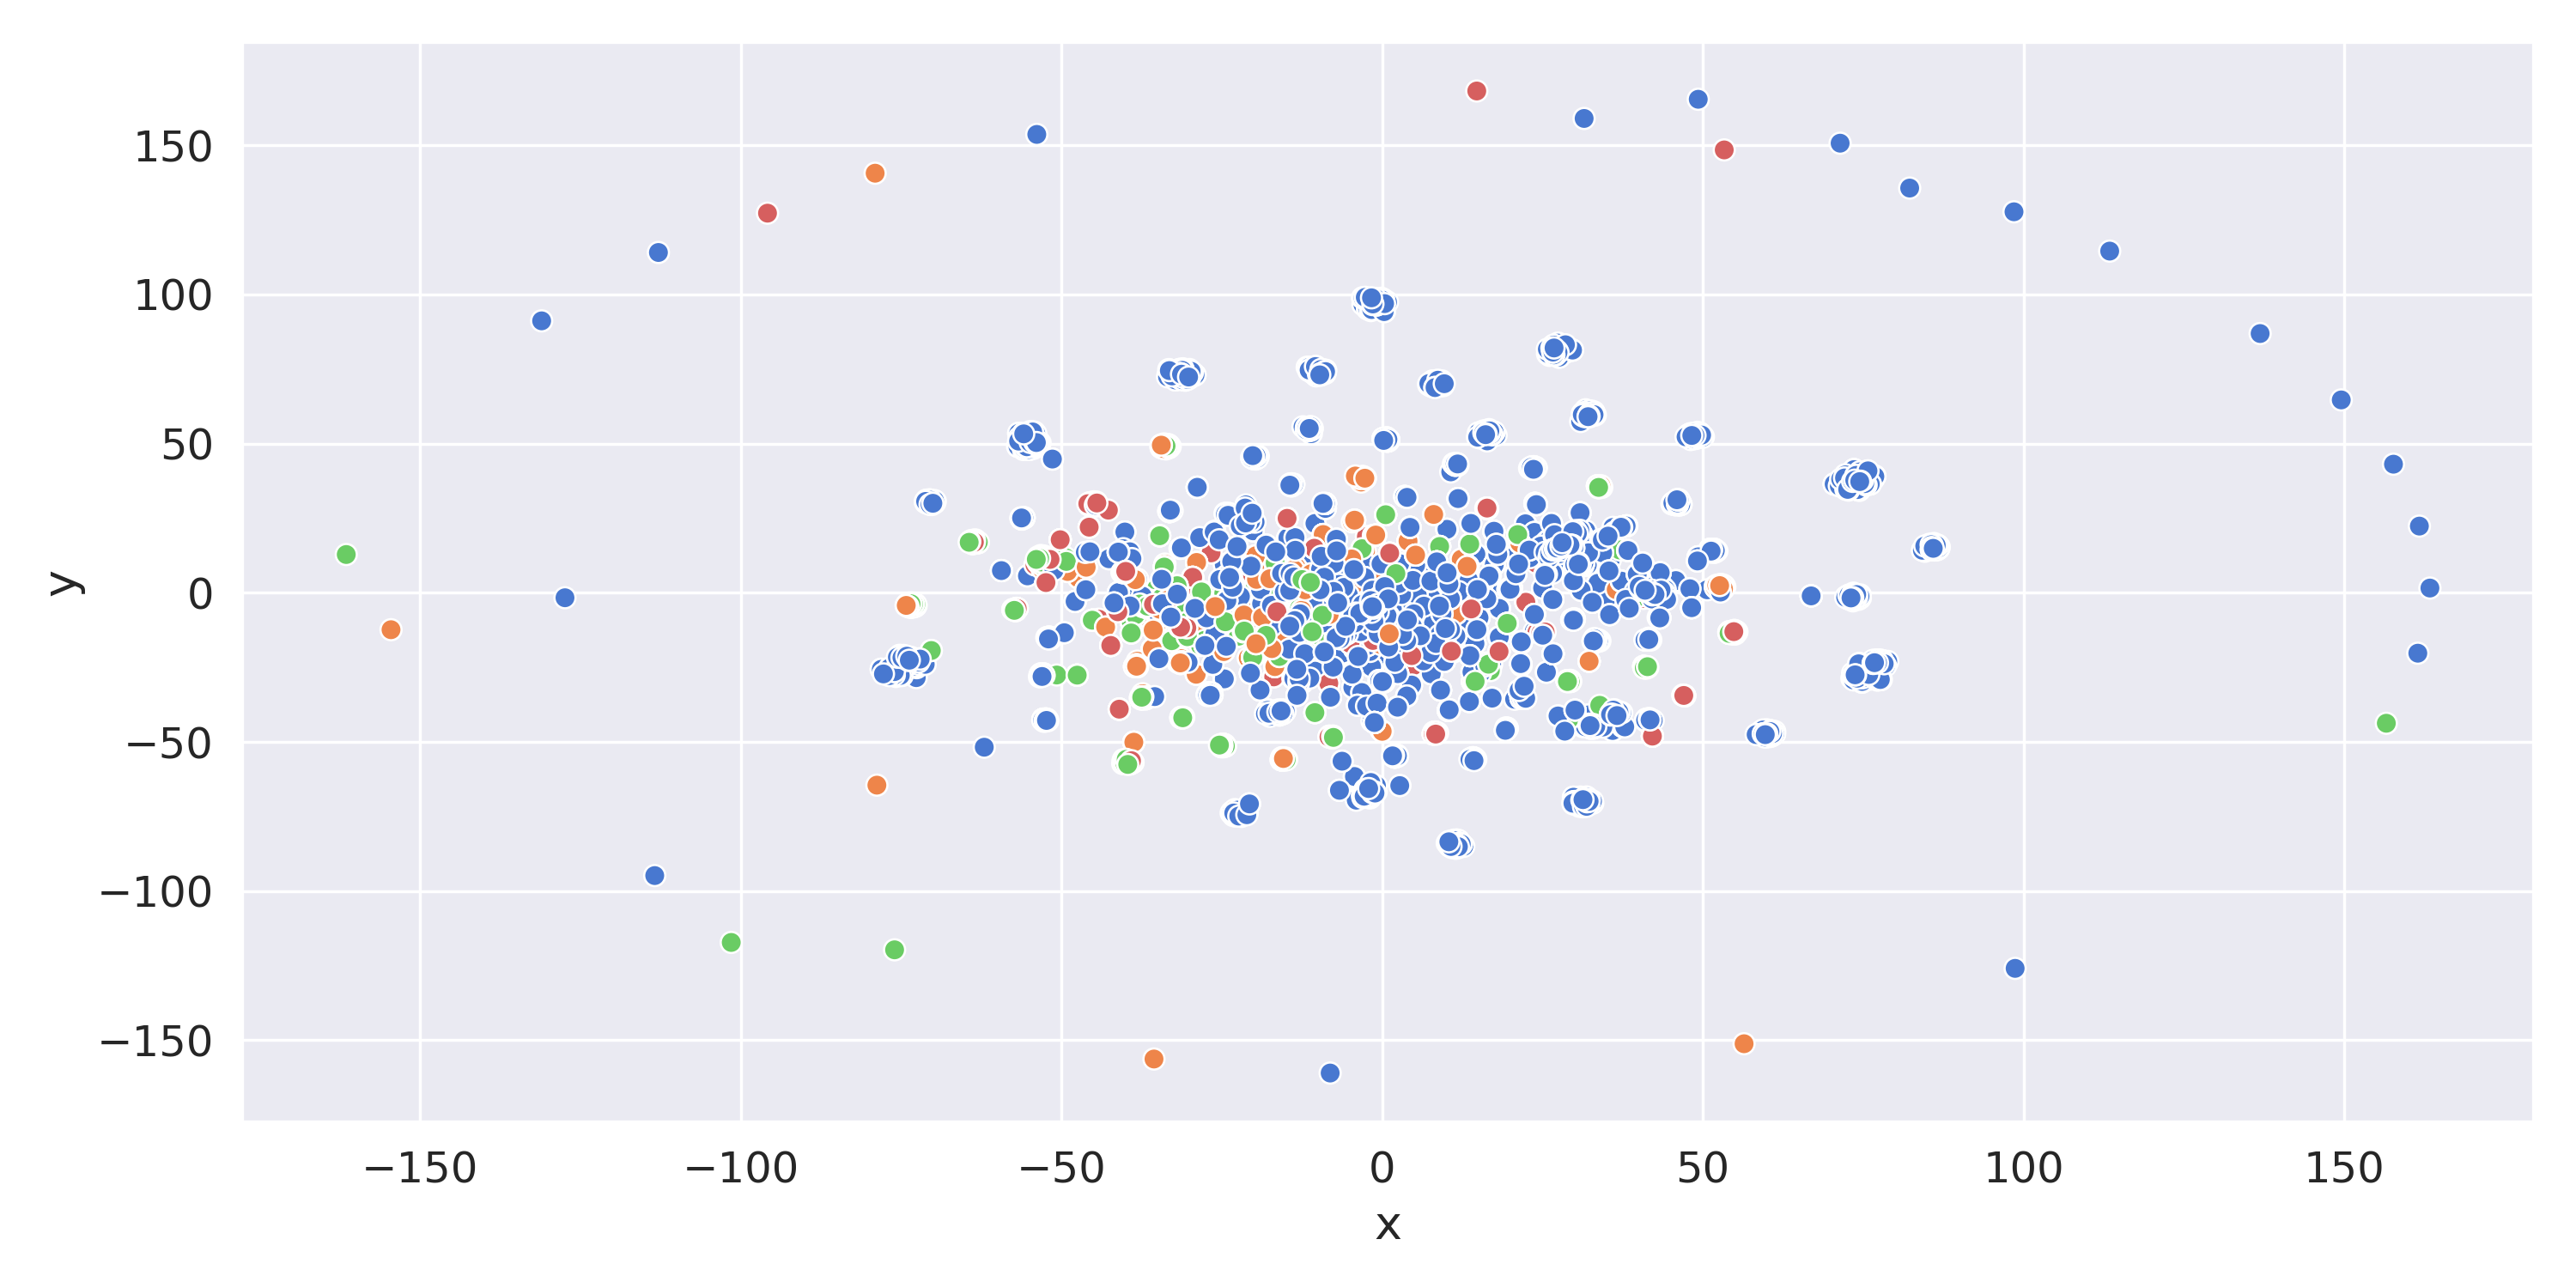
\includegraphics[width=\linewidth]{img/elmo-embeddings-learned.png}
  \caption{Learned ELMo Embeddings 2D}
  \label{fig:sfig1}
\end{subfigure}%
\begin{subfigure}{0.5\linewidth}
  \centering
  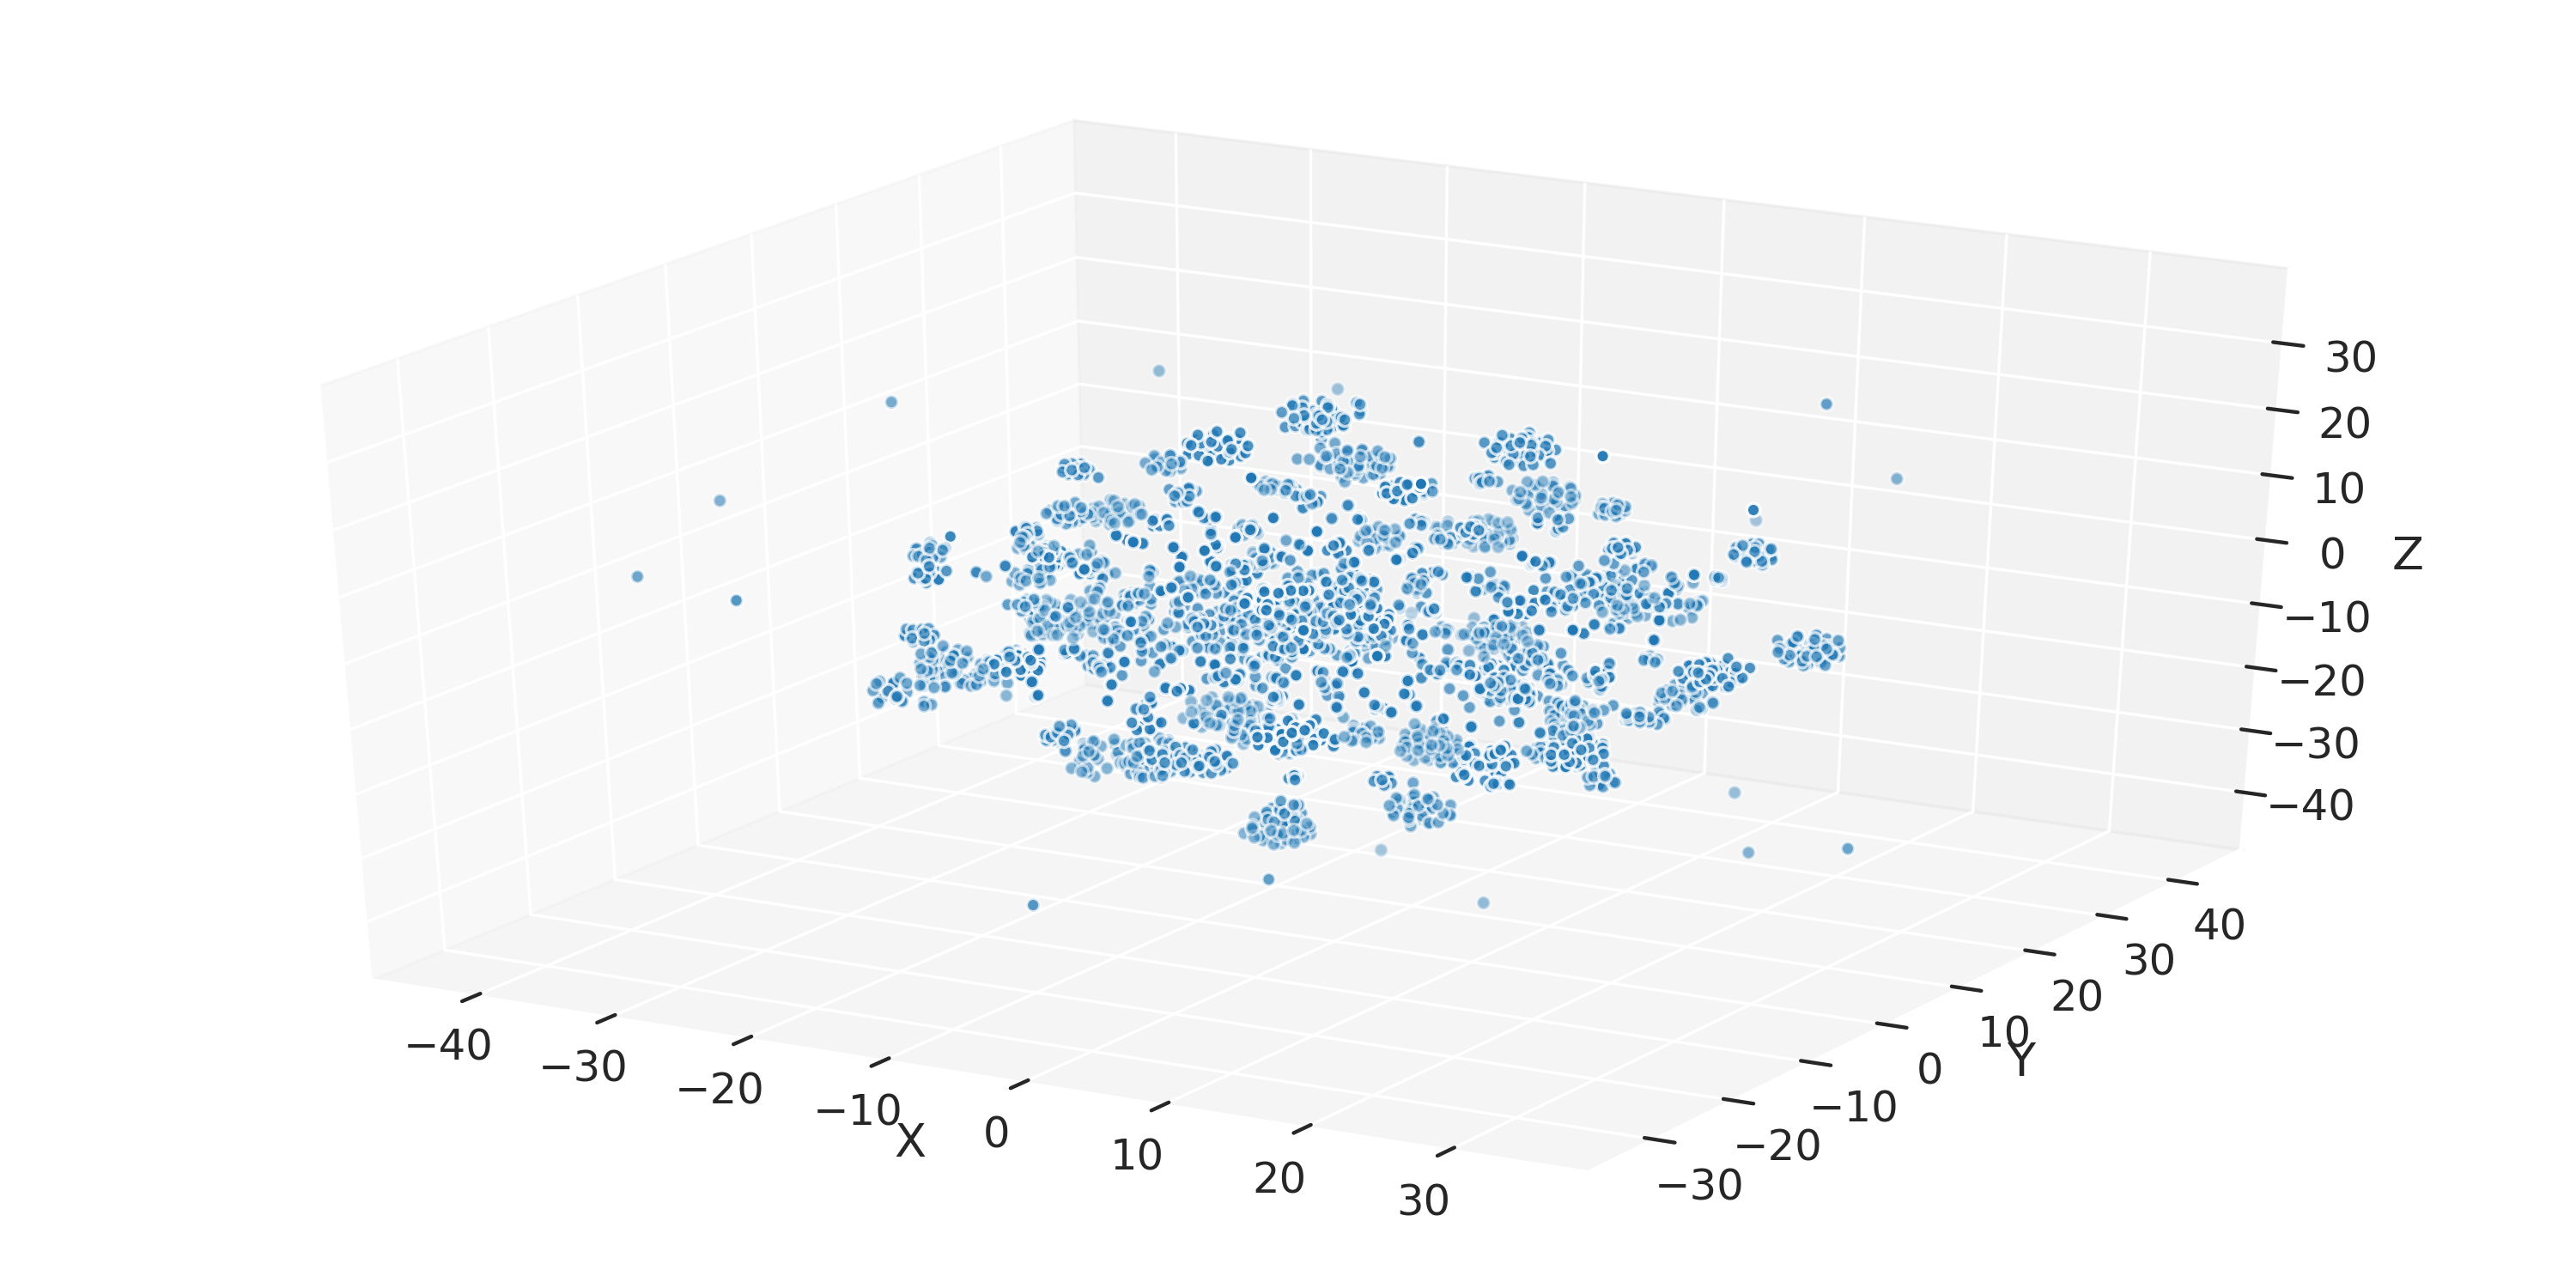
\includegraphics[width=\linewidth]{img/elmo-embeddings-learned-clusters.png}
  \caption{Learned Elmo Embeddings 3D (\textit{movie.title} only).}
  \label{fig:sfig2}
\end{subfigure}
\caption{These plots shows the embeddings representation obtained by learning the ELMo linear combination. Namely, movie.name (blue), actor.name (orange), producer.name (red) and director.name (green). The new ELMo embeddings seems to not have improved the previous situation. However, in higher dimension we notice how the enabled better clusterizations in a 3-dimensional plane.}
\label{fig:fig}
\end{figure*}

\section{Experiments}

We evaluated the models by doing a hyperparameter search by starting from the values used in the original work. We tried to find the hyperparameter combination which maximizes the F1 score over the test dataset. The final results can be seen in Table X.
When using a classical LSTM model, it is possible to see how combining the character representation and the POS/NER additional features lead to results which are better than the default baseline. This happens for all the embeddings considered. Moreover, it seems that the ELMo embeddings provide better performances than the other competitors. 
The BERT embeddings give instead poor results (more than 3\% difference between the F1 mean baseline in some cases).
When using the LSTM-CRF we obtained slightly different results. The LSTM-CRF generally outperforms the simple LSTM model, but here the combination CHAR+NER+POS gives good results only when using the ELMo embedders. By employing BERT or ConceptNet we obtain a better F1 score without using those features (the difference is minimal).
Generally, we also noticed that by making the model learn how to combine the ELMo weightings (elmo-comb) to generate the final embeddings is beneficial for the final performances. Apparently, by fine-tuning the ELMo weightings, it is possible to generate better ``concept clusters" in the embedding space.  Then, the network can effectively learn the hyperplanes which separate each cluster thus leading to less mistagging. [add data about mistagging]
This can be seen from Figure X in which the we show the new 3-dimensional cluster of the ``\textit{movie.name}" concept. 
By using LSTM-CRF and ELMo (learned) we were able to get the best max F1 score of 87.18. Ultimately, the best combination overall with a mean F1 value of  85.99 is obtained by using the ConceptNet embeddings without additional features and the LSTM-CRF model. All these results also surpass the previous baselines obtained with the WFST (83.73).
The models were written in Python and PyTorch by forking from the previous project\footnote{\url{https://github.com/fruttasecca/concept-tagging-with-neural-networks}} and both the code and the dataset are available on Github\footnote{\url{https://github.com/geektoni/concept-tagging-nn-spacy}}.


\section{Conclusion}
The experiments showed us how the usage of the correct embeddings is of utmost importance for obtaining state-of-the-art performances on concept tagging tasks. BERT and ELMo pre-trained models provide new embeddings obtained by looking at the context of the phrase. However, they cannot be used directly out-of-the-box but they need to be fine-tuned on the task at hand to be effective. This can be clearly seen by looking at the difference between the ELMo embeddings created by mere averaging of the layers or by learning the weights of the linear combination. This is also the reason why BERT underperformed in some cases. We used an implementation which extracts directly the embeddings without going through the fine-tuning phase described in the original paper. Therefore, the BERT embeddings are not ``trained" to represent the current concept tagging task. However, the fine-tuning must be done properly to be useful since otherwise we just increase the variance of the results (e.g., the ELMo model showed a higher standard deviation with respect to the other competitors when learning the weights for combining the layers). 
We showed also the impact of adding more features to the original model, more specifically the POS tag and the NER entities. However, we did not see any important improvement. We thought that having extra information like the NER tags could have improved the performances of the models but it was not the case. This process had several issues. For instance, one major problem we found with this method is related to the sparsity of the NER tagging. Over 21000 tokens, only 400~ were tagged with an entity definition (just the 1.9\%). This adds just too little representational power to the original model and therefore it does not produce any huge gain in performances.

\bibliography{acl2019}
\bibliographystyle{acl_natbib}

\end{document}
